\chapter{Introduction}

\newacronym{sm}{SM}{Standard Model}

The quest to understand the universe at its most fundamental level lies at the heart of particle physics. Scientists in this field aim to explore the properties, behaviors, and interactions of elementary particles. Particle physics seeks to answer fundamental questions about the universe, such as the origin of mass, the nature of dark matter, and the unification of forces.

The \acrfull{sm} is a theoretical framework that describes the fundamental particles and their interactions, excluding gravity. It encompasses three of the four known fundamental forces: electromagnetism, the weak nuclear force, and the strong nuclear force. It also incorporates the Higgs mechanism, giving elementary particles their mass. The particles in the Standard Model include quarks, leptons, gauge bosons, and the Higgs boson. Quarks and leptons are the building blocks of matter, while gauge bosons mediate the interactions between these particles.

Particle colliders, key instruments in this research process, accelerate and collide particles to reveal new insights through the analysis of the byproducts of such collisions. These events or processes are characterized by their cross sections. Often denoted as $\sigma$ and measured in units of area, the cross section of an event quantifies the probability of it occurring in a particle interaction. By comparing observed cross sections with those predicted by the \acrshort{sm}, physicists can test the validity of the model and potentially identify discrepancies indicating new physics beyond the \acrshort{sm}.

The performance of particle colliders is determined by two key parameters: the center-of-mass energy and the luminosity, $\mathcal{L}$. While the center-of-mass energy defines the energy scale of the collisions, the luminosity quantifies the rate at which particles interact, directly determining the total amount of events that a collider can produce over a given time period. The instantaneous luminosity, \ilum, is a proportionality constant that relates the rate of an event, $R$, to its cross section, $R = \ilum  \cdot \sigma$. The colossal importance of precise cross section measurements, from which the \acrshort{sm} can be probed, sparks the need for precise measurements of the luminosity and fuels the motivation behind this thesis.

\section{The Large Hadron Collider}
\label{subsec:lhc}

\newacronym{cern}{CERN}{European Organization for Nuclear Research}
\newacronym{lhc}{LHC}{Large Hadron Collider}
\newacronym{ip}{IP}{Interaction Points}
\newacronym{cms}{CMS}{Compact Muon Solenoid}

The \acrfull{lhc} at the \acrfull{cern} is a monumental particle accelerator \cite{lhc}. It's an underground facility spanning the border of France and Switzerland. Its purpose is to accelerate particles beams, one clockwise and the other counterclockwise, and make them collide at high energies to probe the fundamental properties of matter. The collisions happen at four main \acrfull{ip} that correspond to the four main experiments:
\begin{itemize}
	\item \acrfull{cms}: A general-purpose detector designed to investigate a wide range of physics, including the study of the Higgs boson, precision probes of the \acrshort{sm}, and searches for new phenomena. \acrshort{cms} is located at \acrshort{ip} 5.
	\item A Toroidal LHC Apparatus (ATLAS): The second general-purpose detector at the \acrshort{lhc}. Shares similar goals with \acrshort{cms} and is located at the opposite side of the \acrshort{lhc} ring. ATLAS is located at \acrshort{ip} 1.
	\item A Large Ion Collider Experiment (ALICE): A dedicated heavy-ion detector designed to study the physics of strongly interacting matter at extreme energy densities, such as quark-gluon plasma. ALICE is located at \acrshort{ip} 2.
	\item Large Hadron Collider beauty (LHCb): A detector designed to study the differences between matter and antimatter by studying particle interactions involving the "beauty" quark. LHCb is located at \acrshort{ip} 8.
\end{itemize}

The \acrshort{lhc} stands as the world's largest particle accelerator, capable of accelerating protons to a maximum energy of 6.8 TeV. It started operations in 2009 and has since been a cornerstone of particle physics research with its most notable achievement being the discovery of the Higgs boson in 2012 \cite{HiggsDiscovery}.

% Runs, correspond to <insert_here_run_definition> and are also given a unique number. Fill and runs lenghts can vary as well as the number of runs within a given fill.

The \acrshort{lhc} operates according to a planned schedule, which is meticulously planned and updated, when needed, to ensure the success of its experimental programs and upgrades. The current schedule, as shown in \autoref{fig:lhc_schedule}, outlines the activities for Run 3, which is expected to continue until 2025.


\begin{figure}[!htb]
    \centering
    \includegraphics[width=0.8\textwidth]{images/assets/lhc_schedule.png}
    \caption[LHC Run 3 schedule]{The LHC schedule for Run 3, detailing the operational plan until 2025 (from \textit{Ref.} \cite{LHCSchedule}).}
    \label{fig:lhc_schedule}
\end{figure}

\subsection{Accelerator Complex}
\label{subsec:acc_complex}

\newacronym{bcid}{BCID}{Bunch Crossing Identifier}

The \acrshort{lhc} is only the final stage of a complex series of accelerators that prepare the particles for collision. Before protons are injected into the \acrshort{lhc}, they pass through a sequence of smaller accelerators that progressively increase their energy. This series of accelerators forms the comprehensive CERN accelerator complex, as shown in Figure~\ref{fig:cern_acc_complex}.

\begin{figure}[h]
	\centering
	\includegraphics[width=\textwidth]{images/assets/cern_accelerator_complex.png}
	\caption[CERN Accelerator Sequence]{Diagram of the \acrshort{cern} Accelerator Sequence (from \textit{Ref.} \cite{cern-accelerator-complex}): Sequence of accelerators that prepare protons for injection into the \acrshort{lhc}. The path that protons follow can be traced from Linac4, to BOOSTER, to the PS, to the SPS, and finally to the LHC. Highlighted in yellow are the four main experiments at the \acrshort{lhc}. The Linac3 and LEIR, whose purpose is to provide ions for the LHC, are also shown.}
	\label{fig:cern_acc_complex}
\end{figure}

The \acrshort{cern} accelerator complex begins its operations with the Linear Accelerator 4 (Linac4) \cite{Linac4}, which, has served as the primary source for proton beams since 2020. Linac4 boosts the energy of negative hydrogen ions (H$^-$) --- that is, hydrogen atoms with an additional electron --- to 160 million MeV. Using radio frequency (RF) cavities, Linac4 charges a series of conductors in an alternating positive and negative manner, causing the particles to be accelerated. Before being pulsed through the accelerator, the H$^-$ ions are squeezed into a tight beam using quadrupole magnets. These ions are then readied to enter the Proton Synchrotron Booster (PSB), where they lose their two extra electrons and only the protons remain. The PSB further accelerates these protons to 2 GeV, before they proceed to the Proton Synchrotron (PS). At the PS, the proton energy is increased to 26 GeV. Subsequently, the protons are directed to the Super Proton Synchrotron (SPS), where their energy reaches 450 GeV. Finally, these protons are conveyed to the \acrshort{lhc}, where each beam is accelerated to an energy of 6.8 TeV.

In addition to protons, the \acrshort{lhc} also accelerates heavy ions, namely, lead and xenon nuclei. These ions initially enter the Linear Accelerator 3 (Linac3). Once gathered, they are sped up in the Low Energy Ion Ring (LEIR) and eventually follow the same trajectory as the protons to reach their maximum energy.


\subsection{Particle Beams}
\label{subsec:particle_beams_lhc}

In the \acrshort{lhc}, particles are grouped into bunches, each containing approximately $10^{11}$ protons at the start of a physics fill. These bunches travel around a 27 km ring at nearly the speed of light, resulting in an orbiting frequency of approximately 11245.5 Hz. The RF cavities that accelerate the bunches operate with an oscillating electric field at a frequency of 400 MHz, creating a total of 35640 RF buckets, each spaced 2.5 ns apart. This arrangement is demanding, as it requires a high degree of timing resolution for any detector system aiming to obtain measurements per bucket. Buckets are grouped into sets of 10, with only the first bucket nominally filled with particles. This grouping increases the spacing between filled particle bunches to 25 ns. These bunch slots are referred to as bunch crossings and assigned a unique number called \acrfull{bcid}, ranging from 1 to 3564.

Each \acrshort{lhc} fill has a well-defined filling scheme. This scheme provides information on parameters such as the bunch spacing, the number of filled bunches per beam, the number of collisions at each \acrshort{ip}, and the number of consecutive filled bunches, also known as a train, among others. The filling scheme heavily influences the physics conditions of the fill, dictating the experimental environment and collision dynamics. Each fill is uniquely identified by a fill number which is incremented by a counter. Special fills may be requested to study specific experimental conditions in order to achieve the desired physics goals.


\subsection{Compact Muon Solenoid Experiment}
\label{subsec:cms}

The \acrlong{cms} \cite{TheCMSCollaboration_2008}, is a multi-purpose detector operating at the \acrshort{lhc}, designed to operate under high instantaneous luminosity conditions. These conditions require radiation resistance, sub-detector systems with high granularity, and an intricate readout and trigger system. To fulfill its requirements the \acrshort{cms} apparatus is composed of a series of subsystems. Figure~\ref{fig:cms_detector} shows a schematic of the \acrshort{cms} detector and its subsystems. \acrshort{cms} is located underground close to the French village of Cessy, between Lake Geneva and the Jura mountains. Its coordinate system in relation to the \acrshort{lhc} ring is illustrated in Figure~\ref{fig:cms_system_coordinates}.

\begin{figure}[h]
	\centering
	\makebox[\textwidth][c]{%
		\begin{minipage}[b]{0.5\textwidth}
			\centering
			\includegraphics[width=\textwidth]{images/assets/cms_detector.png}
			\subcaption{}
			\label{fig:cms_detector}
		\end{minipage}
		\hspace{0.05\textwidth}
		\begin{minipage}[b]{0.5\textwidth}
			\centering
			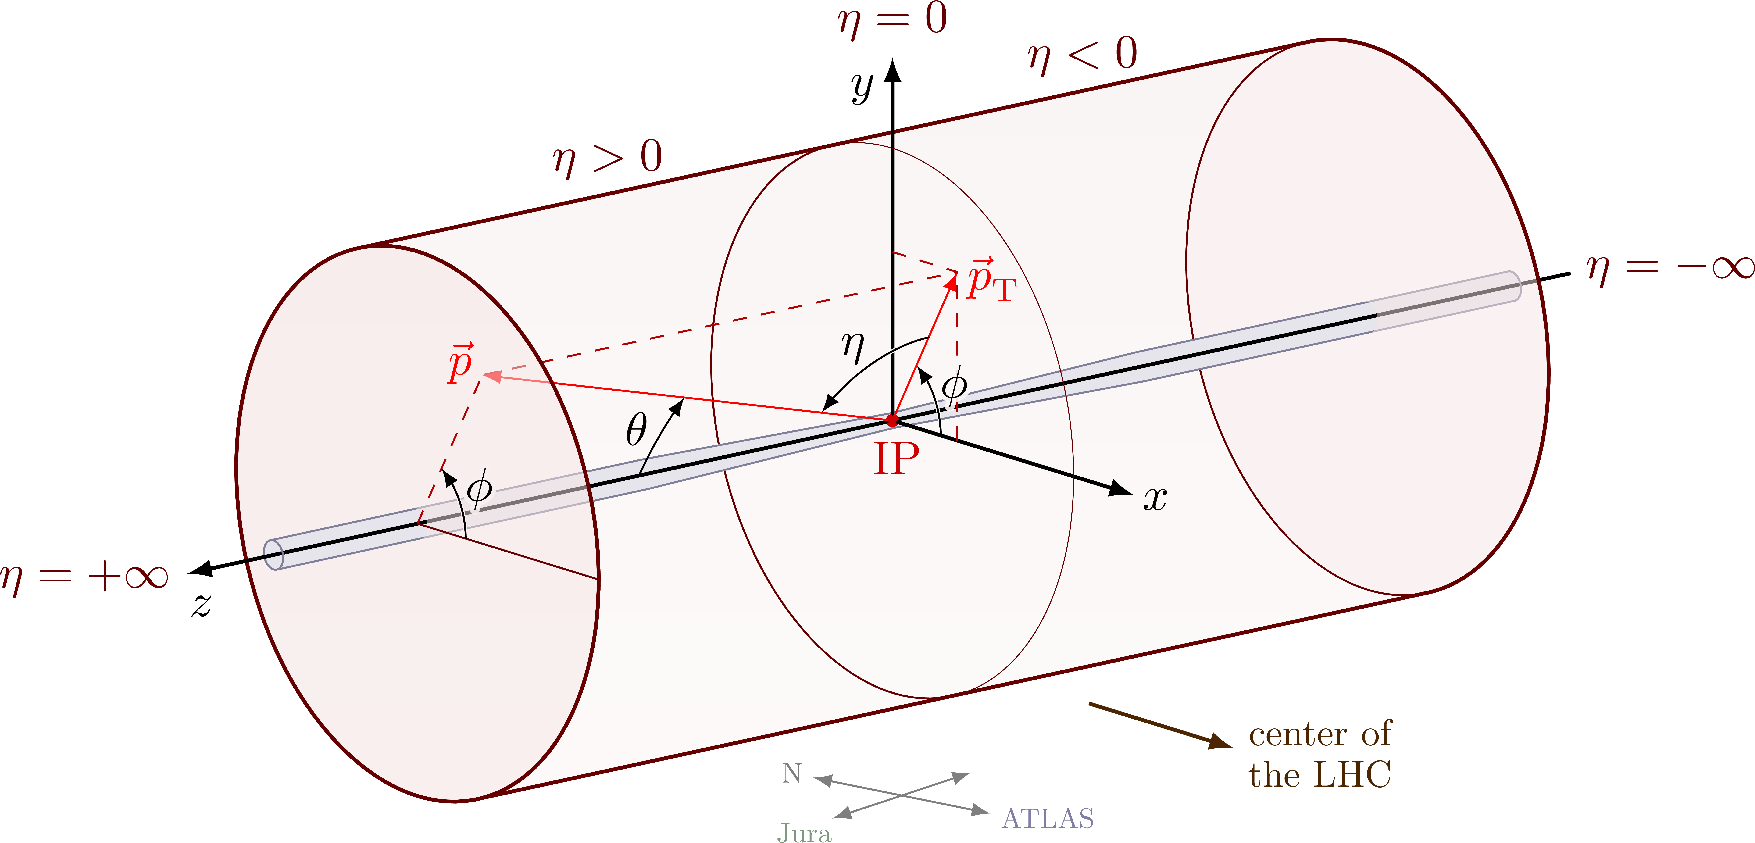
\includegraphics[width=\textwidth]{images/assets/cms_system_coordinates.pdf}
			\subcaption{}
			\label{fig:cms_system_coordinates}
		\end{minipage}
	}
	\caption[CMS detector and coordinate system]{(a) Schematic of the \acrshort{cms} detector outlining its subsystems (adapted from \textit{Ref.} \cite{CERN:39040}). (b) Diagram of the \acrshort{cms} coordinate system as seen with the \acrshort{lhc} cylinder in the background. The $x$-axis points radially to the center of the \acrshort{lhc} ring, the $y$-axis points upwards, and the $z$-axis points along the beam direction. The azimuthal angle, $\phi$, is measured from the $x$-axis to the $\vv{p}_T$ vector in the $x-y$ plane. The polar angle, $\theta$, is measured from the $z$-axis to the $\vv{p}$ vector. Each zone is labeled with the corresponding pseudorapidity, $\eta$, defined as $\eta = - \ln \tan (\theta / 2)$.}
	\label{fig:cms_images}
\end{figure}

As stated in Section~\ref{subsec:lhc}, the \acrshort{cms} physics program encompasses a wide range of topics. From the study of the Higgs boson, to continuously probing the \acrshort{sm} through precision measurements, to searching for new physics phenomena at high energy scales. The detector is built from the conjunction of multiple layers of subsystems, each with a dedicated focus on measuring specific products of the collision events as they traverse the detector. The subsystems, from the center outwards, are depicted in Figure~\ref{fig:cms_slice}.

\begin{figure}[h]
	\centering
	\includegraphics[width=\textwidth]{images/assets/cms_slice.png}
	\caption[Transverse slice of CMS detector]{Transverse slice of the \acrshort{cms} detector (from \textit{Ref.} \cite{Barney:2120661}). The subsystems are shown from the center outwards: the silicon tracker, the electromagnetic calorimeter, the hadronic calorimeter, and the muon system.}
	\label{fig:cms_slice}
\end{figure}

\newacronym{ecal}{ECAL}{Electromagnetic Calorimeter}
\newacronym{hcal}{HCAL}{Hadronic Calorimeter}

The part of the detector closest to the beam pipe is the silicon tracker. This subsystem is composed of silicon sensors that track the paths of charged particles as they ionize the silicon while moving through it. Influenced by the \acrshort{cms} magnet, the curvature of these particles' paths provides crucial information for calculating their momentum, with more curved paths indicating lower momentum. The tracker can reconstruct the paths of charged particles, including electrons, hadrons, and high-energy muons. Immediately following the tracker are the \acrshort{cms} calorimeters: the \acrfull{ecal} and the \acrfull{hcal}. These calorimeters measure the energy of particles by stopping them and measuring the energy they deposit. The \acrshort{ecal}, composed of lead tungstate crystals, detects electrons and photons by scintillating upon interaction with these particles. Photodetectors, designed to operate within the high magnetic field, are attached to the back of each crystal to detect the scintillation light and convert it to an electrical signal that is then amplified and analyzed. The \acrshort{hcal} measures the energy of hadrons, which are particles made of quarks and gluons, such as protons and neutrons. Additionally, it allows for the indirect measurement of non-interacting particles, such as neutrinos, through missing transverse energy, which represents the imbalance in the sum of transverse momentum of the particles in the event. The \acrshort{hcal} is constructed with alternating layers of absorber and scintillating materials, producing rapid light pulses when particles pass through. It is organized into several sections: the barrel (HB), outer barrel (HO), endcap (HE), and forward (HF) sections. Muons, heavy cousins of electrons, are the particles most likely to pass through the calorimeters and reach the muon system. The muon system is the outermost layer of the \acrshort{cms} detector and is designed to detect muons. It is composed of three types of detectors: Drift Tubes (DT), Cathode Strip Chambers (CSC), and Resistive Plate Chambers (RPC). Detailed information on \acrshort{cms} subsystems can be found in \cite{CERN-LHCC-2020-004}.

\section{Luminosity}
\label{sec:luminosity}

Luminosity is essential in particle physics research for two key reasons. First, accurate measurements of instantaneous luminosity are crucial for tracking the performance of both the accelerator and its associated detectors \cite{PhysRevAccelBeams.21.102801}. Second, integrated luminosity often represents the primary source of uncertainty in numerous cross section measurements \cite{cms2022measurement, sirunyan2019measurement}. This section provides a detailed overview of the concept of luminosity.

\subsection{Instantaneous and Integrated Luminosity}
\newacronym{sbil}{SBIL}{Single Bunch Instantaneous Luminosity}

Luminosity is defined as the ratio between the rate of events, $R$, and the cross section of a given process, $\sigma$:
\begin{equation}
    \label{eq:inst-luminosity}
    \mathcal{L} = \frac{R}{\sigma}
\end{equation}
$\mathcal{L}$ has then units of $[\mathrm{area}]^{-1} [\mathrm{time}]^{-1}$ where cm$^{-2}$s$^{-1}$ or fb$^{-1}$s$^{-1}$ are common units ($1$ barn  $= 10^{-28}$ m$^{-2}$). Integrating over a given time interval, $t_2 - t_1$, yields the integrated luminosity, $L$:
\begin{equation}
    \label{eq:int-luminosity}
    L = \int_{t_1}^{t_2} \mathcal{L} dt = \int_{t_1}^{t_2} \frac{R}{\sigma} dt = \frac{N}{\sigma}
\end{equation}
It follows that $L$ is proportional to the number of events, $N$, produced in the collider.

From \autoref{eq:int-luminosity} it can be seen that luminosity can be measured if the cross section of a given process is known. This is the case for lepton colliders, where the ``candle" process $e^+ e^- \rightarrow e^+ e^-$ is used to measure luminosity \cite{Burkhardt:1056691}. However, for hadron colliders, which involve collisions of particles made of quarks, such as protons, this approach is not feasible due to the large uncertainties in the calculation of cross sections. Another approach is to measure luminosity using machine parameters, as described in the next section.

\subsection{Luminosity from Machine Parameters}
\label{subsec:luminosity_from_machine_parameters}

The \acrfull{sbil}, $\mathcal{L}_b$, can be measured using the collider's machine parameters \cite{Burkhardt:1056691}.
\begin{figure}[h]
    \centering
    \includegraphics[width=0.8\textwidth]{images/assets/bunch_crossing.png}
    \caption[Bunch crossing illustration]{Bunch crossing illustration (from \textit{Ref.} \cite{Burkhardt:1056691}).}
    \label{fig:bunch_crossing}
\end{figure}
For colliding bunches containing $N_1$ and $N_2$ particles respectively, the expected value of $\mathcal{L}_b$ is given by the following equation:
\begin{equation}
    \label{eq:sbil-machine-params}
    \mathcal{L}_b = \frac{N_1 N_2 f_{rev}}{A_{eff}}
\end{equation}
In this equation, $f_{rev}$ represents the orbiting frequency around the \acrshort{lhc}, as described in \autoref{subsec:particle_beams_lhc}, and $A_{eff}$ is the effective transverse area where collisions occur, also referred to as the luminous region. If the transverse distribution of particles was uniform, $A_{eff}$ would be equivalent to the transverse bunch overlap. However, considering the transverse particle distributions $\rho_1$ for bunch 1 and $\rho_2$ for bunch 2, the effective transverse area is defined by the overlap integral:
\begin{equation}
    \label{eq:effective-area}
    \frac{1}{A_{eff}} = 2 \int \rho_1(x,y) \rho_2(x,y) dxdy
\end{equation}
The factor of 2 corresponds to the Møller factor, which accounts for the fact that the two bunches are colliding at equal relativistic speeds and in opposite directions \cite{furman2003moeller}. Typically, it is assumed that these transverse particle distributions are uncoupled, meaning: 
\begin{equation}
    \begin{cases}
		\rho_1 \left(x, y \right) = \rho_{1x} \left( x \right) \rho_{1y} \left( y \right) \\
		\rho_2 \left(x, y \right) = \rho_{2x} \left( x \right) \rho_{2y} \left( y \right) \\
    \end{cases}\,.
\end{equation}
Under this assumption, the effective transverse area can be rewritten as:
\begin{equation}
    \label{eq:effective-area}
    \frac{1}{A_{eff}} = 2 \int \rho_{1x}(x) \rho_{2x}(x) dx \times \int \rho_{1y}(y) \rho_{2y}(y) dy = \frac{1}{W_{eff}} \times \frac{1}{H_{eff}}
\end{equation}
Here, $W_{eff}$ and $H_{eff}$ represent the effective transverse width and height, respectively. Substituting this back into equation \ref{eq:sbil-machine-params}, we get:
\begin{equation}
    \label{eq:sbil-machine-params-2}
    \mathcal{L}_b = 2 N_1 N_2 f_{rev} \int \rho_{1x}(x) \rho_{2x}(x) dx \times \int \rho_{1y}(y) \rho_{2y}(y) dy
\end{equation}
Further, assuming that the transverse particle distributions are Gaussian with widths $\sigma_{x1}$, $\sigma_{x2}$ and heights $\sigma_{y1}$, $\sigma_{y2}$, the equation becomes:
\begin{equation}
    \label{eq:sbil-machine-params-3}
    \mathcal{L}_b = 2 N_1 N_2 f_{rev} \int G_x (\sigma_{x1}) G_x (\sigma_{x2}) dx \times \int G_y (\sigma_{y1}) G_y (\sigma_{y2}) dy
\end{equation}
$G_i (\sigma)$ in this context is the Gaussian distribution with standard deviation $\sigma$ in the $i \in {x,y}$ direction and a mean of zero:
\begin{equation}
    \label{eq:gaussian-distribution}
    G_i (\sigma) = \frac{1}{\sigma \sqrt{2 \pi}} e^{-\frac{i^2}{2 \sigma^2}}
\end{equation}
Expanding the first integral:
\begin{equation}
	\label{eq:sbil-machine-params-4}
	\int G_x (\sigma_{x1}) G_x (\sigma_{x2}) dx = \frac{1}{2 \pi \sigma_{x1} \sigma_{x2}} \int e^{-\frac{x^2 \left( \sigma_{x1}^2 + \sigma_{x2}^2 \right)}{2 \sigma_{x1}^2 \sigma_{x2}^2}} dx
\end{equation}
and considering
\begin{equation}
	\int e^{-a x^2} dx = \sqrt{\frac{\pi}{2a}}
\end{equation}
equation \ref{eq:sbil-machine-params-4} can be simplified to:
\begin{equation}
	\label{eq:sbil-machine-params-5}
	\int G_x (\sigma_{x1}) G_x (\sigma_{x2}) dx = \frac{1}{2 \pi \sigma_{x1} \sigma_{x2}} \sqrt {\frac{\pi \sigma_{x1}^2 \sigma_{x2}^2}{\sigma_{x1}^2 + \sigma_{x2}^2}} = \frac{1}{2 \sqrt{\pi} \sqrt{\sigma_{x1}^2 + \sigma_{x2}^2}}
\end{equation}
Using the same approach for the second integral and substituting the results back into equation \ref{eq:sbil-machine-params-3}, we get: 
\begin{equation}
\label{eq:sbil-machine-params-6}
\mathcal{L}_b = \frac{N_1 N_2 f_{rev}}{2 \pi \Sigma_X \Sigma_Y}
\end{equation}
where $\Sigma_X = \sqrt{2\pi} W_{eff} = \sqrt{2\pi} \sqrt{\sigma_{x1}^2 + \sigma_{x2}^2}$ and $\Sigma_Y = \sqrt{2\pi} H_{eff} = \sqrt{2\pi} \sqrt{\sigma_{y1}^2 + \sigma_{y2}^2}$. In the case of round beams, the root-mean-squared widths of the horizontal and vertical beam profiles are equivalent to $\sqrt{\epsilon_{N} \beta^{*} / \gamma}$. $\gamma$ is the relativistic Lorentz factor, and $\beta^{*}$ corresponds to the value of the optical function $\beta$ at the IP. $\epsilon_{N}$ is the normalized transverse emittance, with a values of $3.75\mu m$ for the \acrshort{lhc} \cite{Brüning:782076}.

\subsection{Luminosity Calibration}
\label{subsec:luminosity_calibration}

Luminosity detectors, also called luminometers, are located at the \acrshort{ip}s of the \acrshort{lhc} and measure various observable quantities related to the rate of the collisions. Due to the differences between the luminometers, the nature of their recorded observables, and their location at the \acrshort{cms} cavern, each is assumed to only capture a fraction of the total collisions. This bias in the luminometers is accounted for by a detector-specific calibration factor, the visible cross section, $\sigma_{vis}$. Using equations \ref{eq:inst-luminosity} and \ref{eq:sbil-machine-params-3} this calibration can be expressed as:
\begin{equation}
    \label{eq:vis-cross-section}
    \sigma_{vis} = \frac{2 \pi \Sigma_X \Sigma_Y R}{N_1 N_2 f_{rev}}
\end{equation}
Once calculated for each luminometer, the visible cross section can be used to convert the measured rates to luminosity:
\begin{equation}
    \label{eq:luminosity-from-rates}
    \mathcal{L} = \frac{R}{\sigma_{vis}}
\end{equation}
In both these equations, $R$ represents the measured rate of events from a particular luminometer.

\subsection{Zero-Counting Method}
\label{subsec:zero-counting}

Due to the constraints in the read-out electronics of some luminometers, there's a chance that simultaneous particle hits might be recorded as a single event. This necessitates a more advanced approach to counting hits accurately. It is postulated that the distribution of the number of hits can be modeled by a Poisson distribution \cite{TheLHCbcollaboration_2014} with mean, $\mu$, that is proportional to luminosity.
\begin{equation}
    \label{eq:luminosity-from-hits}
    \mathcal{L}_b = \frac{\mu f_{rev}}{\sigma}
\end{equation}
The zero-counting method consists of calculating the probability that a luminometer records zero hits, $P_0$, regardless of the number of collisions that occur. This probability is given by the following equation:
\begin{equation}
    \label{eq:zero-counting}
    P_0 = \sum_{i=0}^{\infty} \frac{\mu^i e^{-\mu}}{i!} p^i = e^{-\mu(1-p)}
\end{equation}
$\mu$ is the mean number of hits per bunch crossing, also known as pileup, and $p$ is the probability that no observables are recorded in a bunch crossing with $i$ interactions. It then follows that luminosity is proportional to the natural logarithm of $P_0$:
\begin{equation}
    \label{eq:luminosity-from-hits-2}
    \mathcal{L}_b = \frac{\mu f_{rev}}{\sigma} = - \frac{\log (P_0)}{1-p} \frac{f_{rev}}{\sigma} = - \log (P_0) \frac{f_{rev}}{\sigma_{\mathrm{vis}}}
\end{equation}
The value of $p$ is here absorbed into the visible cross section \cite{Sirunyan:2759951} and does not need to be known beforehand.

The zero counting method is not without its limitations. From \autoref{eq:zero-counting} it can be seen that the probability of recording zero hits decreases exponentially with increasing pileup, or similarly, increasing luminosity. This leads to a phenomenon known as ``zero starvation", where the probability of recording zero hits, $P_0$, becomes very small. This can lead to a situation where the luminometer underestimates the number of hits, and consequently, the luminosity.

%%%%%%%%%%%%%%%%%%%%%%%%%%%%%%%%%%%%%%%%%%%%%%%%%%%%%%%%%%%%%%%%%
%% LUMINOMENTER: TO APPROACH AFTER KNOWING WHAT LUMINOISITY IS %%
%%%%%%%%%%%%%%%%%%%%%%%%%%%%%%%%%%%%%%%%%%%%%%%%%%%%%%%%%%%%%%%%%

\section{Luminometers}
\label{subsec:luminosity_detectors}

\newacronym{bril}{BRIL}{Beam Radiation Instrumentation and Luminosity}
\newacronym{plt}{PLT}{Pixel Luminosity Telescope}
\newacronym{bcm1f}{BCM1F}{Fast Beam Conditions Monitor}
\newacronym{4nb}{4NB}{4Nibble}
\newacronym{ls}{LS}{Lumisection}
\newacronym{bib}{BIB}{Beam-Induced Background}


The \acrfull{bril} group is responsible for measuring luminosity at \acrshort{cms}. In addition to this primary task, the group monitors \acrfull{bib}, and dangerous beam loss events that may trigger a beam abort. They also manage beam timing, minimum bias triggers for data acquisition, and the monitoring and simulation of the radiation environment within the \acrshort{cms} cavern. Luminosity is measured with dedicated detectors called luminometers.

These specialized detectors are capable of providing luminosity measurements with a per-bunch timing granularity. At \acrshort{cms}, the number of events measured by most of these systems are integrated over $2^{14}$ \acrshort{lhc} orbits, which corresponds to $\approx 1.458$ s. This amount of time is referred to as a \acrfull{4nb}. Another interval of integration often used during luminosity analysis is the \acrfull{ls} and corresponds to 16 $\times$ \acrshort{4nb} ($\approx 23.311$ s).

Since these detectors usually operate during long periods of time, four quantities are used to identify a particular operation period. These correspond to: a fill number, synchronized across all \acrshort{lhc} experiments; a run number, incremented multiple times in a fill as needed by the \acrshort{cms} data acquisition system; a \acrshort{ls} number, unique to \acrshort{cms} and resetting at the start of every run; and a \acrshort{4nb}, also unique to \acrshort{cms} and resetting at the start of every lumisection.

Figure~\ref{fig:cms_bril_detectors} shows the \acrshort{cms} location of some the systems operated by the \acrshort{bril} group.

\begin{figure}[h]
	\centering
	\includegraphics[width=\textwidth]{images/assets/cms_bril_detectors.png}
	\caption[BRIL systems at CMS]{Systems operated by BRIL group at the Compact Muon Solenoid experiment.Green text indicates, that the instrumentation has been rebuilt for Run 3 (from \textit{Ref.} \cite{Saariokari:2826125}).}
	\label{fig:cms_bril_detectors}
\end{figure}

For a detector to be used as a luminometer, it must meet certain essential requirements. One of the most critical use cases for luminometers is their ability to provide online instantaneous luminosity. This capability is crucial for the operation of the \acrshort{lhc} and the goals of the \acrshort{cms} experiment. Additionally, having per-bunch granularity is important, as the calibration process for the luminometers heavily depends on the available statistics, as will be addressed in \autoref{subsec:the_van_der_meer_scan_methodology}.

Two other characteristics of paramount importance are the stability of the detector over long periods of time and linear response to varying experimental conditions. The former is necessary to ensure that the luminometers can provide reliable measurements throughout the entire period of operations. A luminometer’s stability is typically affected by its accumulated radiation dose, which decreases the detector’s efficiency over the course of the data taking period. In order to adjust the detector’s response, several adjustments are made to its operating configuration.

The latter characteristic concerns how the detector’s response changes under different experimental conditions. In current LHC conditions, the pileup is at its highest near the start of the fill. As the fill progresses, the natural decay of the beam population, commonly referred to as ``luminosity burn-off", causes the pileup to decrease. A luminometer’s response to these changes in pileup conditions must be as linear as possible with respect to luminosity. Additionally, changes in the filling scheme can affect the detector’s response, as some detectors are more sensitive to ``afterglow" effects, where the signal from a previous bunch crossing is still present in the immediately adjacent bunch crossings. Similar to maintaining the detector's stability, the linearity of the luminometer’s response can be preserved through corrective procedures, which will be discussed in \autoref{subsec:extrapolation_of_vdM_calibration} and with focus on 2023 data in \autoref{ch:2023_luminosity_calibration}. The ``online" visible cross section and linearity correction may be updated periodically to compensate for changes in the detector's efficiency and linear behavior.

The following subsections will describe the luminometers that were considered for this work, their positions within the \acrshort{cms} detector, and how the luminosity is extracted from their observable measurements.

\subsection{Hadron Forward}
\newacronym{hf}{HF}{Hadron Forward}
\newacronym{hfoc}{HFOC}{Hadron Forward Occupancy Count}
\newacronym{hfet}{HFET}{Hadron Forward Transverse Energy}

As stated in \autoref{subsec:cms}, the \acrshort{cms} \acrshort{hcal} is composed of several sections, one of which is the \acrfull{hf} calorimeter \cite{CMS:2012tda}. The \acrshort{hf} is constructed from quartz scintillators embedded in steel absorbers and is located at $z \pm 11.2$m from the \acrshort{ip}, covering a pseudorapidity range of $3 < |\eta| < 5$. This range allows for better detection of missing transverse energy, which is crucial for probing the \acrshort{sm} and searching for new physics phenomena.

The \acrshort{hf} calorimeter uses Photomultiplier Tubes (PMTs) to collect Cherenkov light produced by particles passing through the quartz scintillators. A dedicated readout system collects these signals and converts them into luminosity measurements using two methods. The \acrshort{hfoc} method tracks the fraction of bunch crossings with no energy deposition above a threshold in specific \acrshort{hf} towers ($\eta$ rings 31 and 32). The average number of these counts is then converted to luminosity via the zero-counting method.

The \acrshort{hfet} method, was implemented in 2016. It is based on the assumption that the measured transverse energy sum is proportional to the luminosity. This assumption is used to estimate the number of particles depositing signals and convert it to luminosity. The HFET method is used in parallel with the HFOC method to cross-check the luminosity measurements.

\subsection{The Pixel Luminosity Telescope}
\label{subsubsec:plt}

One of the dedicated luminosity detectors is the \acrfull{plt} \cite{CMS-DP-2021-020}. This detector is based on the use of silicon pixel sensors, 48 in total, arranged in groups of 3 in a telescope-like structure. The sensors are placed at a distance of $1.75$m from both ends of the \acrshort{ip} at a $|\eta| \approx 4.2$, nearly parallel to the beam line. Figure~\ref{fig:cms_plt} shows the a diagram for the 48 sensors and the half of the detector with the mounting support.

\begin{figure}[H]
	\centering
	\includegraphics[width=\textwidth]{images/assets/cms_plt.png}
	\caption[PLT detector telescopes]{\textbf{Left}: Picture illustrating eight telescopes of the \acrshort{plt} detector, which correspond to half detector (from \textit{Ref.} \cite{Romeo:2797807}). \textbf{Right}: One quarter of the full \acrshort{plt} detector with mounting support and with visible connections to the readout electronic (from \textit{Ref.} \cite{DelannoySotomayor:2765247}).}
	\label{fig:cms_plt}
\end{figure}

The \acrshort{plt}'s silicon sensors are bump bonded to PSI46v2 readout chips \cite{KASTLI2006188}, which offer two readout modes: the "fast-or" mode allows for a readout rate of 40MH$z$, allowing per bunch measurements. A \acrshort{plt} ``track" is registered when a particle passes through all 3 sensors of a telescope, referred to as a ``triple coincidence". The full pixel data readout mode reads at a lower rate of 3.3 kH$z$ being useful for other studies. This method allows for track reconstruction which helps discern between particles from the collision and background noise. Figure~\ref{fig:plt_triple_coincidence} shows an illustration of a triple coincidence.

\begin{figure}[H]
	\centering
	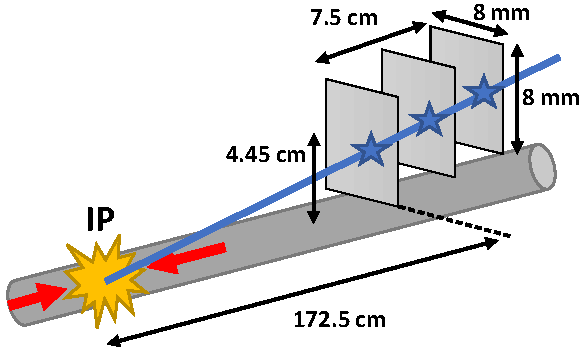
\includegraphics[width=0.5\textwidth]{images/assets/TripleCoincidenceSketch.pdf}
	\caption[Triple coincidence in PLT]{Illustration of a triple coincidence in the \acrshort{plt} detector. A hit is considered when a particle passes through the 3 sensors of a telescope (from \textit{Ref.} \cite{Lujan:2797692}).}
	\label{fig:plt_triple_coincidence}
\end{figure}

The zero-counting method, described in \autoref{subsec:zero-counting}, is used to convert the number of hits to luminosity. For PLT, the zero starvation effect is usually not a problem, as the typical PLT occupancy is on the order 0.1-0.2 triple coincidences per telescope per bunch crossing at high luminosity conditions.

\subsection{The Fast Beam Conditions Monitor}

The \acrfull{bcm1f} \cite{CMS-DP-2022-033} can measure not only the luminosity, but also the \acrshort{bib}. It consists of 24 double-pad silicon sensors arranged in four semi-circles, referred to as ``C-shapes", positioned 7.2 cm from the beam pipe and at a distance of 1.8 m on either side of the \acrshort{ip}. This placement allows for the separation of incoming and outgoing particles, corresponding to a flight time of 6.25 ns for particles traveling at relativistic speeds. This setup enables the discernment of signals originating from collisions, \acrshort{bib}, and noise caused by the activation of surrounding material \cite{Zagozdzinska_2016}. \autoref{fig:bcm1f_real_life} shows the arrangement of one of the C-shapes.

\begin{figure}[h]
\centering
\includegraphics[width=\textwidth]{images/assets/bcm1f_real_life.png}
\caption[BCM1F sensor arrangement]{Arrangement of the six sensors in one of the C-shapes of the \acrshort{bcm1f} detector (from \textit{Ref.} \cite{DelannoySotomayor:2809025}).}
\label{fig:bcm1f_real_life}
\end{figure}

\newacronym{vme}{VME}{Versa Module Europa}
\newacronym{rhu}{RHU}{Realtime Histogramming Unit}

A particle passing through the bulk of a silicon sensor will ionize the material, creating electron-hole pairs. These pairs are then separated by an electric field, generating a current pulse proportional to the energy of the particle. The signals detected in the sensors are read by two parallel systems. The older back-end system utilizes the \acrfull{vme} standard and was the primary system during Run 2. The newer $\mu$TCA-based system began operation in Run 3 \cite{Karacheban:2294183}.

The \acrshort{vme} back-end system discriminates signals using a constant threshold, and the hits are sent to a \acrfull{rhu}. The hits per bunch are then converted to luminosity using the zero-counting method. The $\mu$TCA system employs a more sophisticated approach, using a peak-finding algorithm that counts pulses based on the signal's derivative and amplitude. This method not only allows for more accurate distinction between hits and noise but also enables the detection of simultaneous hits by analyzing the pulse shape. Both systems, BCM1F and BCM1FUTCA, are used as independent luminometers.

\subsection{Pixel Cluster Counting}

A large number of modules from the \acrshort{cms} Pixel detector is also used as a luminometer. Upgraded in 2017, it consists of four barrel layers, BPIX, and three disks, FPIX, on each side of the \acrshort{ip} at distances of 291, 396, and 516 mm, respectively. The BPIX is made up of a total of 79 million pixels in 1184 modules, while the FPIX contains 45 million pixels in 672 modules. The layouts of the two detectors, the original and the upgraded one, are compared in \autoref{fig:pcc_layout}. Further details on the design and construction of the upgraded Pixel detector can be found in \cite{tracker2020cms}.

\begin{figure}[h]
\centering
\includegraphics[width=\textwidth]{images/assets/pcc_upgrade.png}
\caption[Upgraded pixel detector]{Longitudinal view of the Phase 1-upgraded pixel detector compared to the original detector layout (from \textit{Ref.} \cite{tracker2020cms}). Labels L1 to L4 indicate the barrel layers, while D1 to D3 indicate the disks.}
\label{fig:pcc_layout}
\end{figure}

The Pixel Cluster Counting (PCC) method counts the mean number of clusters, a conglomerate amount of charged particle hits, in the pixel detector in zero-bias events (events from nominally colliding bunch crossings without any specific activity requirement). The mean number of clusters, averaged over several measurements, can be expressed as

\begin{equation}
	\label{eq:pcc-clusters-mean}
	\langle N_{\text{clusters}} \rangle = \langle N_{\text{clusters} / \text{interaction}} \rangle \cdot \frac{\sigma_{\text{minBias}}}{f_{rev}} \cdot \mathcal{L}_b
\end{equation}

from which the PCC calibration factor can be calculated as $\sigma_{\text{vis}} = \sigma_{\text{minBias}} \cdot \langle N_{\text{clusters} / \text{interaction}} \rangle$ where $\sigma_{\text{minBias}}$ is the proton-proton cross section for minimum bias events. The $\langle N_{\text{clusters}} \rangle$ is measured by averaging the number of clusters over \acrshort{ls} intervals with a 0.1\% statistical uncertainty for orbit integrated luminosity.

Due the large amount of pixels used, the probability of one pixel being hit by two charged particles from the same bunch crossing is extremely small. The PCC method has been shown to provide stable and linear luminosity measurements and was used as the primary luminometer for the \acrshort{cms} experiment in previous years \cite{Sirunyan:2759951}. The measurements from this detector are only used during the offline analysis. 

\subsection{Drift Tube}
\label{subsec:dt}

Located in the \acrshort{cms} muon system, the Drift Tube (DT) is a sub-system of the muon barrel (MB) that provides an estimate of the number of muon tracks passing through the detector. This estimate, done with the Barrel Muon Track Finder (BMTF) algorithm \cite{Triossi_2017}, is assumed to be proportional to the luminosity which allows for DT to be used as a luminometer. However, it does not provide luminosity measurements with per bunch granularity, but is rather \acrshort{ls}-integrated. These limitations make the measurement of its calibration factor, $\sigma_{\text{vis}}$, dependent on the other luminometers. However, due to its good stability and linearity, it is often calibrated to match other luminometers as a way to compare for stability and linearity.

%%%%%%%%%%%%%%%%%%%%%%%%%%%%%%%%%%%%%%%%%%%%%%%%%%%%%%%%%%%%%%%%%
%% LUMINOMENTER: TO APPROACH AFTER KNOWING WHAT LUMINOISITY IS %%
%%%%%%%%%%%%%%%%%%%%%%%%%%%%%%%%%%%%%%%%%%%%%%%%%%%%%%%%%%%%%%%%%
